\chapter{Introduction}
\label{chap:Intro}
This report describes the design and implementation of a hardware accelerator that performs the Sobel operator on an 8-bit monochrome image. It represents the work that is performed during the laboratory exercise "Edge detection design project" \cite{Sparsoe2014} in the DTU course 02203 - Design of Digital Systems.\\
In section \ref{sec:AccDesign} and \ref{sec:Optimization}, two different designs are presented. One design is trading speed for fewer resources, the other favours speed over resources. The two designs have been implemented in VHDL and simulated with ModelSim v.10.3. The implemented VHDL code is synthesized for the Spartan6 using the Xilinx ISE 14.7 software. Hardware tests are performed on the Nexys3 develeopment board from Digilent Inc. The performance of the different approaches, in terms of throughput and FPGA area, are evaluated and discussed in chapter \ref{chap:Results}.

\section{System overview}
\label{sec:SysOverview}
Figure \ref{fig:SysArch} shows an overview of the system architecture. The input image is stored in external RAM and the output image is written back to the external RAM, but at a different memory location. Using the to two signals 'start' and 'finish', a four phase handshake protocol is used to start and finish the processing sequence.

\begin{figure}[H]
	\centering
	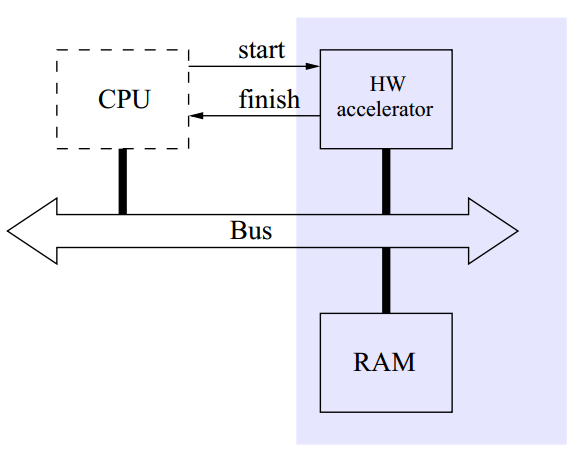
\includegraphics[width=0.5 \textwidth]{SystemArchitecture.png}
	\caption{System architecture as given by the lab assignment \cite{Sparsoe2014}.}
	\label{fig:SysArch}
\end{figure}
